\section{однофазный мостовой АИН}
\ctikzset{tripoles/Lnigbt/height=1.4}
\ctikzset{tripoles/Lnigbt/width=0.8}
\begin{circuitikz}
	\foreach \x\y\NN in {0/3.75/1, 0/1.25/2, 4/3.75/3, 4/1.25/4} {
	\draw ({\x},{\y}) node[Lnigbt,bodydiode,label={[above left=0.05cm and 0.5 cm]\tiny{VT\NN}}] (vt\NN) {} 
		       node[label={[above right=-0.2cm and 0.3 cm]\tiny{VD\NN}}] {};
	}

	\draw (vt1.source) -- (vt2.drain) node[midway] (LoadL) {};
	\draw (vt3.source) -- (vt4.drain) node[midway] (LoadR) {};
	\node (LoadC) at ($(LoadL)!0.5!(LoadR)$) {};

	\draw (LoadL) to[R,l={$R_\textcyrillic{н}$},*-] (LoadC) to[L,l={$L_\textcyrillic{н}$},-*] (LoadR);


	\draw[dashed] (barycentric cs:vt1={0.9*0.3},vt2={0.9*0.7},vt3={0.1*0.3},vt4={0.1*0.7}) -- 
	(barycentric cs:vt1={0.1*0.3},vt2={0.1*0.7},vt3={0.9*0.3},vt4={0.9*0.7}) -- 
	(barycentric cs:vt1={0.1*0.8},vt2={0.1*0.2},vt3={0.9*0.8},vt4={0.9*0.2}) --
	(barycentric cs:vt1={0.9*0.8},vt2={0.9*0.2},vt3={0.1*0.8},vt4={0.1*0.2}) -- cycle;
	
%        \path let \p1 = (vt1.drain) in node  at (-2, \y1) {B};
	\draw ([xshift=-4.5cm]vt1.drain) -- (vt3.drain);
	\draw ([xshift=-4.5cm]vt2.source) -- (vt4.source);
	\draw ([xshift=-2.1cm]vt1.drain) to[R,l=\tiny{R1}] ([xshift=-2.1cm]LoadL) to[R,l=\tiny{R2}] ([xshift=-2.1cm]vt2.source);
	\draw ([xshift=-2.8cm]vt1.drain) to[C,l_=\tiny{C1}] ([xshift=-2.8cm]LoadL) to[C,l_=\tiny{C2}] ([xshift=-2.8cm]vt2.source);
	\draw ([xshift=-2.8cm]LoadL.center) to[short,*-*] ([xshift=-2.1cm]LoadL.center);
                        
	\draw[<-,>=latex] (-0.2, 2.4) -- (-1.3,-0.5) node[below] {ноль не подключен};
\end{circuitikz}

Мостовая схема состоит из двух нулевых. Напряжение на нагрузке в 2 раза больше чем в нулевой. Лучше используется источник питания. Форма напряжения и токов одинакова с нулевой схемой.

Напряжения гармоник $U_{(n)} = \frac{2\sqrt{2}}{\pi(2k-1)}U_\textcyrillic{п} \Rightarrow U_1 = \frac{2\sqrt{2}}{\pi}U_\textcyrillic{п} $.

Стоимость СПП $\approx$ току.
Надо экономить ток. Если взяли СПП -- получите максимальное напряжение.

В инверторах нужны конденсаторы на большое напряжение $>500$В, Нужно конденсаторостроение
на 300-350-400-450 В. Если действующее напряжение 220В, то амплитудное 311В. А если 380В --
амплитуда больше 500В. Рассматриваем схему, где ноль не подключен.
Линейное напряжение равно 380В. Чему равно $E_{d0}=513$ -- это среднее при нагрузке,
амплитуда Х.Х. (холостого хода) когда конденсатор зарядится максимально 537В, а если скачет на 10\%
то 600В. Принято выбирать с запасом 15-20\%. 1.75 Коэффициент запаса

Запорожье поставляло 80\% ПП в СССР.

\begin{tikzpicture}
\draw (0,1.5) node[nigbt] {$VT_1$} 
	(1.5,0) node[nigbt] {$VT_4$}
	(1,1.5) node[right] {включены нормально};

\draw[thin]	(6,0.75) -- (6,1.75)
	(6,0.75) --++(2,0)
	(6,0) --++(2,0) (6,0) node[left] {$-U_\text{п}$};
\draw[thin,dashed] (7,1.5) -- (5.8,1.5) node[left] {$U_\text{п}$};
\draw[thick] (7,0.75) -- (7,1.5) -- (8,1.5) -- (8,0.25);
\end{tikzpicture}

Напряжение и ток одного знака -- ток течет через транзисторы, если разных -- ток течет черещ диоды.

Акцентируем внимание: Если сделаем недостаточно большую паузу. Момент выключения --
максимум тока. У электромагнитного поля тоже есть масса как у автомобиля. Чтобы быстро 
поменять направление нужен сверлегкий автомобиль.
\begin{figure}[ht!]
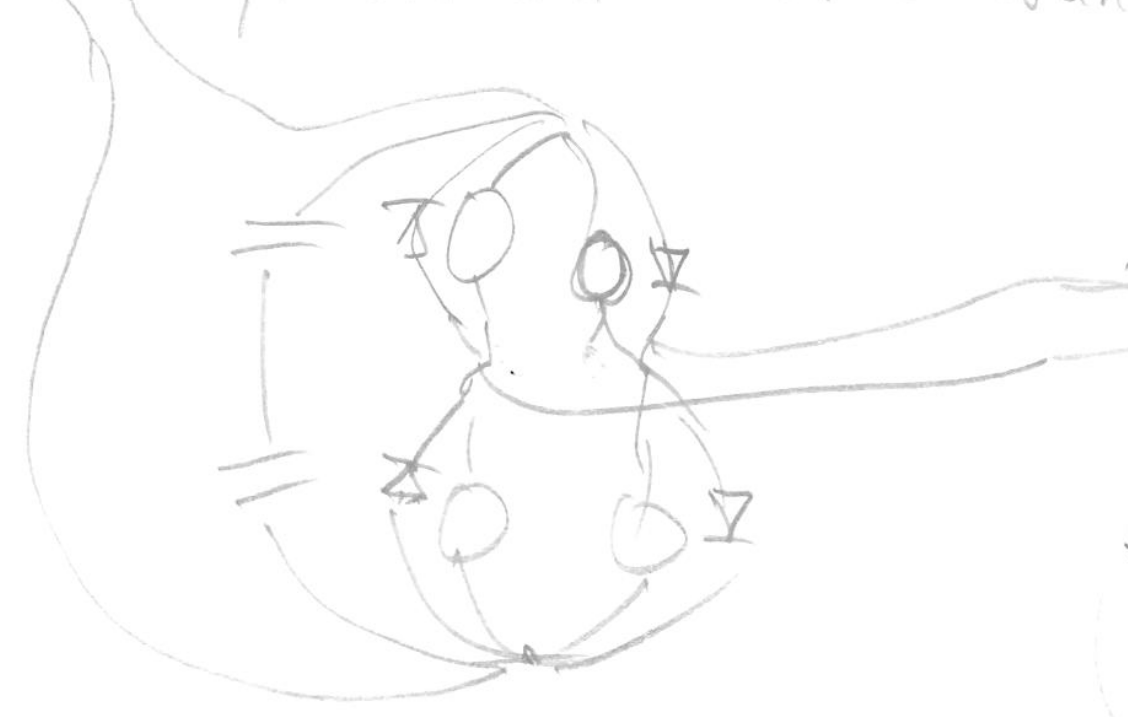
\includegraphics[scale=0.2]{real_lection12b1.png}
	\caption{длина проводов}
\end{figure}

\begin{figure}[ht!]
\begin{circuitikz}
\ctikzset{tripoles/Lnigbt/height=1.4}
\ctikzset{tripoles/Lnigbt/width=0.8}
        \foreach \x\y\NN in {0/3.75/1, 0/1.25/2, 4/3.75/3, 4/1.25/4} {
	\draw[thin] ({\x},{\y}) node[Lnigbt,bodydiode,label={[above left=0.05cm and 0.5 cm]\tiny{VT\NN}}] (vt\NN) {}
                       node[label={[above right=-0.2cm and 0.3 cm]\tiny{VD\NN}}] {};
        }
        \draw[thin] (vt1.source) -- (vt2.drain) node[midway] (LoadL) {};
	\draw[thin] (vt3.source) -- (vt4.drain) node[midway] (LoadR) {};
        \node (LoadC) at ($(LoadL)!0.5!(LoadR)$) {};

	\draw[ultra thick] (LoadL.center) --++ (0.7,0) node (LoadLL) {}; 
	\draw[ultra thick] (LoadR.center) --++ (-0.7,0) node (LoadRR) {};
	\draw[thin] (LoadLL.center) to[R,l={$R_\textcyrillic{н}$},*-] (LoadC) to[L,l={$L_\textcyrillic{н}$},-*] (LoadRR);


%        \draw[dashed] (barycentric cs:vt1={0.9*0.3},vt2={0.9*0.7},vt3={0.1*0.3},vt4={0.1*0.7}) --
%        (barycentric cs:vt1={0.1*0.3},vt2={0.1*0.7},vt3={0.9*0.3},vt4={0.9*0.7}) --
%        (barycentric cs:vt1={0.1*0.8},vt2={0.1*0.2},vt3={0.9*0.8},vt4={0.9*0.2}) --
%        (barycentric cs:vt1={0.9*0.8},vt2={0.9*0.2},vt3={0.1*0.8},vt4={0.1*0.2}) -- cycle;

%        \path let \p1 = (vt1.drain) in node  at (-2, \y1) {B};
	\draw[ultra thick] ([xshift=-4.5cm]vt1.drain) -- ([xshift=-2.8cm]vt1.drain);
	\draw[thin] ([xshift=-2.8cm]vt1.drain) -- (vt3.drain);
	\draw[ultra thick] ([xshift=-4.5cm]vt2.source) --  ([xshift=-2.8cm]vt2.source);
	\draw[thin] ([xshift=-2.8cm]vt2.source) --(vt4.source);
	\draw[thin] ([xshift=-2.1cm]vt1.drain) to[R,l=\tiny{R1}] ([xshift=-2.1cm]LoadL) to[R,l=\tiny{R2}] ([xshift=-2.1cm]vt2.source);
	\draw[thin] ([xshift=-2.8cm]vt1.drain) to[C,l_=\tiny{C1}] ([xshift=-2.8cm]LoadL) to[C,l_=\tiny{C2}] ([xshift=-2.8cm]vt2.source);
	\draw[thin] ([xshift=-2.8cm]LoadL.center) to[short,*-*] ([xshift=-2.1cm]LoadL.center);
\end{circuitikz}
	\caption{провода, выделенные жирным, могут быть длинными, остальные -- короткими}
\end{figure}

Магнитное сопротивление -- длина проволоки. Периметр - длина
\begin{circuitikz}
\draw (0,0) rectangle (1,0.1);
\end{circuitikz}
много больше чем у круглого проводника
\begin{circuitikz}
\draw (0,0) -- (1,0) (0,0.2) -- (1,0.2);
\draw [thin,->]  (0,0.12) --  (-0.1,0.12) arc(-90:-270:0.12) --++(0.1,0);
\draw [thin,->]  (0,0.08) --  (-0.1,0.08) arc(90:270:0.12) --++(0.1,0);
\draw [thin,->]  (1,0.12) --  (1.1,0.12) arc(-90:90:0.12) --++(-0.1,0);
\draw [thin,->]  (1,0.08) --  (1.1,0.08) arc(90:-90:0.12) --++(-0.1,0);
	\draw (1.5,0) node[right] {магнитное поле};
\end{circuitikz}

Я не открыл другую пару, а напряжение стало отрицательным. И открыла диоды ЭДС самоиндукции. Это надо понимать. Я могу не спешить 
открывать пару транзисторов. Все равно проводят диоды.

\subsection*{Способы регулирования выходного напряжения однофазного АИН}
Схема похожа на 4-х квадрантный ИППН. Реверсивный выпрямитель = ИППН. 

А если быстро переключать, то постоянное напряжение переходит в переменное. Онофазный ИППН должен долго поддерживать протекание тока.
Нулевая схема не подходит для ИППН. В ИППН было $\tau$ разные, а здесь $\tau = T - \tau$. Первая гармоника (постоянный ток) не нужен.

Как регулирвать величину? Способы:

1) Путем изменения $U_\text{П}$ (входного постоянного напряжения) с больной стороны на здоровую. Сделать управляемый выпрямитель
можно с помощью ИППН.
4-x квадрантный ИППН может поменять напряжение? Нет! Перепутать диоды. А я хочу регулировать самим инвертором.

2) В мостовой схеме путем неодновременного включения транзисторов.
Можно как и в ИППН постоянно открыть один из транзисторов. 4-й останется работать. Ток будет протекать по КЗ контуру
через индуктивность. Напряжение на нагрузке будет равно 0. Будет включен транзистор и диод (1-й транзистор и 3-й диод
или 40й транзистор и 2-й диод).

\begin{circuitikz}
\draw[thin,->,>=latex] (0,-2) -- (0,2) node[left] {$U_\text{П}$};
\draw[thin,->,>=latex] (0,0) -- (6,0);
	\draw[help lines, smooth] (0,0) -- (0,1.8) -- (1.2,1.8) -- (1.2,0) -- (1.5,0) -- (1.5,-1.8) -- (2.7,-1.8) -- (2.7,0) -- (3,0) -- (3,1.8) -- (4.2,1.8)
	-- (4.2,0) -- (4.5,0);
	\path[pattern=north east lines,fill opacity=5,opacity=0.2] (1.2,0) rectangle (1.5,1.8);
	\path[pattern=north east lines,fill opacity=5,opacity=0.2] (2.7,0) rectangle (3,-1.8);

	\draw[thin,<->] (0,1.5) -- (1.5,1.5) node[midway, above] {$T/2$};
	\draw[thin,<->] (1.5,-0.7) -- (3,-0.7) node[midway, below] {$T/2$};
        \draw[thin,<->] (3,1.65) -- (4.2,1.65) node[midway, above] {$\tau/2$};

	\draw[<-] (1.35,1.3) --++ (1.2,1.5) node[right] {потерялась площадка};

	\draw[domain=0:1.2] plot(\x,{1.8-3.6*exp(-1.7*\x)});
	\draw[domain=1.2:6,dashed,thin] plot(\x,{1.8-3.6*exp(-1.7*\x)});
	\newcommand{\YY}{(1.8-3.6*exp(-1.7*1.2))}
	\draw[domain=1.2:1.5] plot(\x,{ (1.8-3.6*exp(-1.7*1.2))*exp(-0.8*(\x-1.2))});
	\newcommand{\YYY}{(1.8-3.6*exp(-1.7*1.2))*exp(-0.8*(1.5-1.2))}
	\draw[domain=1.5:6,dotted,thin] plot(\x,{ (1.8-3.6*exp(-1.7*1.2))*exp(-0.8*(\x-1.2))});
	\newcommand{\YYYY}{ (2*(1.8-3.6*exp(-1.7*1.2))*(exp(-1.7*(2.7-1.5)-0)) -1.65)}
	\draw[domain=1.5:2.7]  plot(\x,{ 2*(1.8-3.6*exp(-1.7*1.2))*(exp(-1.7*(\x-1.5)-0)) -1.65});
	\draw[domain=2.7:6,dashed,thin]  plot(\x,{ 2*(1.8-3.6*exp(-1.7*1.2))*(exp(-1.7*(\x-1.5)-0)) -1.65});
	\draw [domain=2.7:3] plot (\x, {-\YY*exp(-0.8*(\x-2.7))});
	\draw [domain=3:6,dotted,thin] plot (\x, {-\YY*exp(-0.8*(\x-2.7))});
%	\draw [domain=3:4.2]  plot (\x, {2*\YYYY*exp(-1.7*(\x-3)-0) + 2});
	\draw [domain=3:4.2]  plot (\x, {2.15*\YYYY*exp(-2.2*(\x-3)-0) + 1.76});
	\draw [domain=3:6,dotted,thin]  plot (\x, {2.15*\YYYY*exp(-2.2*(\x-3)-0) + 1.76});
\end{circuitikz}

Уменьшается и среднеквадратичная и средняя.

Домашнее задание: Определить значение 1-й основной гармоники. Высшие гармоники все вместе взятые при $\tau < T/2 $
я покажу как взять.
Положительный импульс - пауза - отрицательный импульс - пауза. Получить выражение, чтобы туда входила $\tau$.

\subsection*{Другие способы:}

Способ ШИР (Широтно импульсного регулирования). Это уже был простейший способ ШИРа. В общем случае -- формирование 
положительных и отрицательных полуволн. Может состоять из нескольких импульсов, которые я могу изменять,
ширина которых изменяется.

Принципиально возможно бесчисленное число способов ШИР, которые отличаются друг от друга количеством импульсов
в каждой полуволне, их полярностью, последовательностью изменения продолжительности отдельных импульсов
и интервалов между ними.

\begin{circuitikz}
\draw[thin,->] (0,-1.5) -- (0,1.5);
	\draw (0,1.2) -- (0.5,1.2) -- (0.5,0) -- (0.7,0) -- (0.7,1.2) -- (1.5,1.2) -- (1.5,0) -- (1.7,0) --
	(1.7,1.2) -- (2.5,1.2) -- (2.5,0) -- (2.7,0) --  (2.7,1.2) -- (3.4,1.2) --  (3.4,0) -- (3.8,0) -- (3.8,-1.2)
	-- (4.5,-1.2) -- (4.5,0) -- (4.7,0) -- (4.7,-1.2) -- (5.5,-1.2) -- (5.5,0) -- (5.7,0) -- (5.7,-1.2) --
	(6.5,-1.2) -- (6.5,0)  -- (6.7,0) -- (6.7,-1.2) -- (7.4,-1.2) -- (7.4,0) -- (7.6,0); 
\end{circuitikz}

Если хватит быстродействия -- предоставляете какие бесконечные возможности. Зря усложнять не нужно. 
При каждом включении-выключении -- потери на транзисторах -- КПД портится, нагрев транзистора.

Хочу чтобы коэффициент ${\displaystyle \frac{U_n}{U_1}}$ было наименьшим. Средне квадратичное 
$I_\eta= {\displaystyle \sqrt{ \sum\limits_{n>1}^\infty U^2(n)} }$ -- за исключением первой гармоники
$ {\displaystyle \frac{I_\eta}{I_1}}$ -- попытаемся сделать поменьше. О них поговорим позже.

Частным случаем ШИР является ШИМ при котором обеспечивается улучшение формы выходного напряжения АИН
за счет уменьшения уровня высших гармоник.

\begin{circuitikz}
	\draw (0.7,0) -- (0.9,0) -- (0.9,-1.2) -- (1.4,-1.2) -- (1.4,0) -- (1.8,0) -- (1.8,-1.2) -- (2,-1.2) -- (2,0) --
	(2.4,0) -- (2.4,1.2) -- (2.6,1.2) -- (2.6,0) -- (3,0) -- (3,1.2) -- (3.4,1.2) -- (3.4,0) -- (3.6,0) -- (3.6,1.2) --
	(4.2,1.2) -- (4.2,0) -- (4.3,0) -- (4.3,1.2) -- (5.3,1.2) -- (5.3,0) -- (5.4,0);  % 4.8 - 180 градусов
	\draw[domain=0:6,help lines, smooth] plot (\x, {-1.4*cos(180*\x/4.8)});
	\draw[thin,->] (0,-1.5) -- (0,1.5);
	\draw[thin,->] (0,0) -- (6.5,0);
	\draw[red] (2.2,0.2) -- (2.8,0.2) -- (2.8,0.6) -- (3.5,0.6) -- (3.5,1.1) -- (4.25,1.1) --(4.25,1.15) -- (5.35,1.15);
	\draw[<-] (4.95, 1.3) --++ (1,1) node[right] {приближение среднего значения к синусоиде};
\end{circuitikz}

Как ШИР так и ШИМ могут быть как одно-полярные так и много-полярные. Наиболее часто с постоянной шириной импульсов.
ШИР (меняется ширина), ЧИР -- частотно импульсная (ширина одинаковая, меняется частота следования)

Для ИППН
$$
U_\text{н} = U_\text{пит} \frac{\tau}{T}
$$

$$
\begin{array}{lll}
	\tau& -& var\\
	T& -&const
\end{array}
\Rightarrow F= const \text{-- ШИР}
$$

$$
\begin{array}{lll}
        \tau& -& const\\
        T& -&var
\end{array}
\Rightarrow F = var \text{-- ЧИР}
$$
Одинаковая амлитуда.

3-й способ, комбинированный -- все способы импульсной модуляции(одинаковая амплитуда).


Известен еще один способ регулирования напряжения АИН путем суммирования на нагрузке напряжений двух АИН
путем суммирования на нагрузке напряжений двух АИН при изменении фазового угла между ними.

\begin{circuitikz}
	\draw (0,0) node[transformer] (B) {}  (-0.6,0) node {U2}
	(B.inner dot A1) node[circ]{}
	(B.inner dot B1) node[circ]{}
	(0,2) node[transformer] (A) {} {}  (-0.6,2) node {U1} 
        (A.inner dot A1) node[circ]{} 
        (A.inner dot B1) node[circ]{}
	(B.A1) -- (A.A2)
	(1,1.2) rectangle (3,2.8)  (2,2)  node {АИН1}
	(1,-0.8) rectangle (3,0.8)  (2,0)  node {АИН2}
	(B.B1) --++ (0.4,0)
	(B.B2) --++ (0.4,0)
	(A.B1) --++ (0.4,0)
        (A.B2) --++ (0.4,0)
	(-2,-0.1) rectangle (-1,2.1)
	(-1.5,1) node[rotate=90] {нагрузка}
	(A.A1) -| (-1.5,2.1)
	(B.A2) -| (-1.5,-0.1)
	(4,-1) -- (4,3)
	(4.5,-1) -- (4.5,3)
	(3,1.7) -- (4,1.7)  (3.4,1.5) node {$-$}
	(3,2.3) -- (4.5,2.3) (3.4,2.5) node {$+$}
	(3,-0.3) -- (4,-0.3)  (3.4,-0.5) node {$-$}
        (3,0.5) -- (4.5,0.5) (3.4,0.7) node {$+$}
;\end{circuitikz}

Проще пояснить на трансформаторах. Включу последовательно. С одинаковой частотой переключаю трансформаторные пары, отличающиеся 
фазовым сдвигом относительно друг друга.

\begin{circuitikz}
\newcommand{\D}{3}
\newcommand{\DD}{1.4}
	\newcommand{\fii}{40}
	\newcommand{\fio}{40}
	\draw[->] (0,0) -- (0,{\D}) node(A) {} node[left] {$U_1$};
	\draw[->] (0,0) -- ({\D*cos(\fii)},{\D*sin(\fii)}) node[right] {$U_2$};
	\draw[thin,dashed] (A.center) --++ ({\D*cos(\fii)},{\D*sin(\fii)}) node(B) {};
        \draw[->] (0,0) -- (B.center);
	\draw ({\DD*cos(65)},{\DD*sin(65)}) arc(65:90:{\DD}) node[midway,above] {$\varphi/2$};

	\draw[thin] (3,0) -- (6,0) 
	(3,0) -- (3,2) -- (4.5,2) --  (4.5,0);
	\draw[thin,dashed] (3.5,0) --  (3.5,1.8) -- (5,1.8) -- (5,0);  
	\draw[domain=3:4.5] plot(\x, {2*sin((\x-3)/1.5*180)});
	\draw[dashed,domain=3.5:5] plot(\x, {1.8*sin((\x-3.5)/1.5*180)});
;\end{circuitikz}

$$
|U_1| = |U_2| = |U|
$$

$$
U_\text{вых} = U_\text{нагр} = 2U Cos\frac{\varphi}{2}
$$

при $\varphi=0$ напряжение сложится. 
